\chapter{Experimental Setup}
\label{sec:expt}
\chaptermark{Experimental Setup}

\begin{center}
\begin{footnotesize}
{\it{``I'm going to find it and I'm going to destroy it. I don't know how yet. Maybe dynamite."}}\\
Steve Zissou, ``The Life Aquatic with Steve Zissou"
\end{footnotesize}
\end{center}

\section{The Large Hadron Collider}
\label{sec:LHC}

In Sec.~\ref{sec:introduction}, we saw that although the Standard Model was tested robustly before the LHC turned on, the Higgs boson had not yet been discovered and there are still unanswered questions not covered under the Standard Model that should lead to new physics. For many decades, the primary tool of discovery in experimental particle physics has been the particle accelerator. In rudimentary terms, two particles are accelerated towards each other and the byproducts of their collisions are studied to look for new particles.

There are two categories of particle accelerators, leptonic and hadronic: leptonic colliders have electron-positron collisions while hadronic colliders use proton-proton or proton-antiproton collisions. As discussed in Sec.~\ref{sec:FundParticles}, protons are made up of a sea of different particles with varying energies, making it difficult to know the exact initial conditions of a collision. A leptonic collider, on the other hand, can tune the initial energy of the collisions to a precise value with strictly designed initial conditions. However, as argued in Sec.~\ref{sec:findinghiggs} and \ref{sec:findingBSM}, the proposed particles could take many energy values, so any search must be done over a wide range, which encourages the use of hadronic collisions. Furthermore, this energy range should explore unprobed regions out of reach of previous detectors. The highest energy collision before the LHC were at the Tevatron at Fermilab which had a maximum center-of-mass energy up to about 2 TeV (2000 GeV).

The Large Hadron Collider was designed with these characteristics in mind: a 27-kilometer circular accelerator for proton-proton\footnote{Heavy ions can also be accelerated in the LHC, leading to interesting research for the strong force, but this is outside the scope of this thesis.} collisions that can reach up to energies of 14 $\rm{TeV}$. An earlier proton-proton accelerator, the Super Proton Synchrotron which found direct evidence for the $Z$ boson~\cite{Arnison:1983rp,Arnison:1983mk,Bagnaia:1983zx}, initializes the proton bunches at 450 $\rm{GeV}$ for injection into the larger ring. Once reaching the LHC, a series of 1232 superconducting dipole magnets with radio frequency cavities increase the energy of the protons as they move around the ring. As these bunches accelerate, the protons will tend to diffuse, so thousands of additional magnets (quadrupole, octopole, etc) are installed to focus the beam. Each bunch in the LHC contains $1.15\times10^{11}$ protons and every run contains 2808 bunches. These high populations are required to probe the highest energies and rarest interactions expected at the LHC.

To quantify how rare an event is, physics utilizes the concept of \textit{cross section} ($\sigma$). This is best illustrated by comparing protons in a bunch to a flow of ballbearings: as two bunches pass through one another, the likelihood that any ballbearing strikes another is proportional to their size, literally their cross-sectional area. Similarly, in quantum physics, the likelihood of an event is determined by its cross section, typically written in units of \textit{barns} (b) where $1$ $\mathrm{b}$ $=$ $10^{-28}$ $\mathrm{m}^2$. The processes intended to be probed at the LHC have cross sections ranging from the order of picobarns ($1$ $\mathrm{pb}$ $=$ $10^{-12}$ $\mathrm{b}$) to fractions of femtobarns ($1$ $\mathrm{fb}$ $=$ $10^{-15}$ $\mathrm{b}$).

Particle accelerators use \textit{luminosity} ($\mathcal{L}$) to indicate how many events of a given cross-section should be expected per second, i.e. $\frac{dN}{dt}=\mathcal{L}\times\sigma$. The luminosity can be defined in terms of the accelerator's parameters:
\begin{equation*}
\mathcal{L} = \frac{\gamma f k_{B}N_p^2}{4\pi \epsilon_{n} \beta^{*}}F
\end{equation*}
where $\gamma$ is the Lorentz factor corresponding to how fast the particles are moving, $f$ is the frequency that bunches revolve through the LHC, $k_{B}$ is the number of bunches, $N_p$ is the number of protons in a bunch, $\epsilon_n$ (normalized transverse emittance) and $\beta^{*}$ (betatron function at the point of interaction) both relate to the physical size of the beam, and $F$ is a reduction factor caused by the crossing angle of the beams. Relevant design parameters are also found in Table~\ref{tbl:LHCLumi}. Ultimately, the design luminosity of the LHC is $\mathcal{L} = 10^{34}$ $\mathrm{cm}^{-2}\mathrm{s}^{-1}$ which corresponds to about 1 billion proton-proton interactions per second. To quantify the total amount of data collected by a particle detector, time-integrated luminosity, in units of $fb^{-1}$, is used to gauge how many events of a given cross-section should be expected. For example, with 10 $\mathrm{fb}^{-1}$ of data, one would expect 10 events for a cross-section of 1 $\mathrm{fb}$.

\begin{table}[htp]
\begin{center}
\begin{tabular}{|c|c|c|}
\hline
Number of bunches & $k_B$ & 2808 \\
\hline
Number of protons/bunch & $N_p$ & $1.15\times10^{11}$ \\
\hline
Bunch separation & & 25 ns \\
\hline
%Betatron Function at IP & $\beta^{*}$ & 0.55 m \\
%\hline
%Normalized Transverse Emittance & $\epsilon_n$ & 3.75 $\mu\mathrm{m}$ \\
%\hline 
Design Luminosity & $\mathcal{L}$ & $10^{34}$ $\mathrm{cm}^{-2}\mathrm{s}^{-1}$ \\
\hline
\end{tabular}
\caption{Design Parameters of the LHC}
\end{center}
\label{tbl:LHCLumi}
\end{table}%

After reaching the desired energy, the proton bunches can interact at four crossing points. Each of these points is the site of a detector on the LHC: CMS (The \textbf{C}ompact \textbf{M}uon \textbf{S}olenoid), ATLAS (\textbf{A} \textbf{T}oroidal \textbf{L}HC \textbf{A}pparatu\textbf{s}), ALICE (\textbf{A} \textbf{L}arge \textbf{I}on \textbf{C}ollider \textbf{E}xperiment), and LHCb (\textbf{LHC} \textbf{b}eauty Experiment). CMS and ATLAS are general detectors for proton-proton interactions, while ALICE and LHCb use the protons to collide with heavy-ion targets to look deeper into the intricacies of the strong force. The remainder of this chapter will detail CMS and how it is used to search for particles like the Higgs.

\section{Our Setting: The Compact Muon Solenoid}
\label{sec:CMS}

The Higgs Boson and theorized particles in BSM physics are expected to be unstable and rapidly decay to particles of the Standard Model, so it's unsurprising that the design requirements of the CMS are built around accurately detecting these particles and characterizing their energies and momenta. To collect the most information about these events, a detector should be designed to record all decay chains so that the full kinematics could be reconstructed. This is the idea behind a \textit{hermetic} detector: different subsystems are nested to capture information about any particle observed and characterized by what sub-detectors they interact with. A detailed view of the CMS detector is seen in Figure~\ref{fig:ExplodedCMS}. This section will overview the subsystems, where further details are found in the CMS Technical Design Reports~\cite{CMSTDR:Vol1,CMSTDR:Vol2}.

\begin{figure}[htbp]
\begin{center}
\includegraphics[width=.9\linewidth]{Experiment/figures/ExplodedCMS.pdf}
\caption[The CMS Detector with Sub-Detector Systems]{The CMS detector is built around a superconducting solenoid, with the muon system (Sec.~\ref{sec:MuonSystem}) on the outer shell. Inside the solenoid, the silicon tracker and pixel detector (Sec.~\ref{sec:Tracker}) are at the innermost radii, with the calorimeter systems (Sec.~\ref{sec:ElecCalo} and \ref{HadrCalo}) are close to the solenoid. Two human figures are used for scale.}
\label{fig:ExplodedCMS}
\end{center}
\end{figure}

\subsection{Coordinates and Conventions for the CMS}
\label{sec:CoordinateConventions}

To unambiguously define locations for components or events found in the detector, a standard coordinate system is used such that the origin is centered at the nominal collision point. In cartesian coordinates, the $y$-axis is defined to be vertically upward while the $x$-axis is points toward the center of the LHC accelerator ring. However, given that the detector is cylindrically symmetric, directions are commonly defined using $\phi$ and $\eta$. $\phi$ is the azimuthal angle starting from the $x$-axis in the $x-y$ plane. $\eta$ is the \textit{pseudorapidity} where $\eta=-\ln[\tan(\theta/2)]$, $\theta$ being the polar angle measured from the $z$-axis. Momentum and energy are then broken into their transverse (away from the axis, e.g. $p_T,E_T$) and longitudinal (along the axis, e.g. $p_z,E_z$) components. Given that the beam is very near the axis and would cause a sizable background, particles that have large $p_T$ or $E_T$ (or in the case of searching for energy imbalance, $E_T^{miss}$) should be the easiest to identify unambiguously.

\subsection{Subsystems in CMS}
\label{sec:CMSSubsystem}

\subsubsection{The Magnet}
\label{sec:Magnet}

One way to categorize the decay products of a particle is to look at their charges. Any charged particle will have a curved trajectory in a magnetic field, where the direction of curvature is determined by the sign of the charge and its scale is proportional to the momentum. Given the large energies and desired precision of the momenta, the magnetic field must be very strong and consistent. CMS uses a 12.9m long, 5.9m in diameter superconducting solenoid with a designed field strength of 4T, about 100,000 times that of the Earth's magnetic field. An iron return yoke, running through the muon system, is used to guide and return the field. In doing so, the magnetic field in the muon system will be antiparallel and of lower magnitude than the field in the calorimeters and tracking systems.

\subsubsection{Muon System}
\label{sec:MuonSystem}

Muons are one of the cleanest signatures to identify and thus crucial for finding new physics. For charged particles, electrons are common byproducts of many low energy decays and can be stopped in dense material. Tau leptons are much rarer, but have a very short lifetime and thus decay in the inner detector. Quarks cannot be observed individually. Neutrinos aren't charged and very difficult to detect as they only interact via the weak force. Muons, on the other hand, are charged, heavy leptons that have long enough lifetimes to pass through the outer reaches of the detector. Because of these properties\footnote{For exactly the same reason, this is why the LHC is deep underground. Cosmic rays commonly hit the Earth's atmosphere and shower particles to the surface. Although nearly all particles can be shielded without much material, decay in the upper atmosphere, or very rarely interact with matter, muons will commonly penetrate the surface and need hundreds of meters of depth to suitably reduce this background.}, muons that come from collisions are measured from three different sub-systems to accurately measure their kinematics. 

\begin{figure}[htbp]
\begin{center}
\includegraphics[width=.7\linewidth]{Experiment/figures/MuonSystem.pdf}
\caption[Arrangement of Detectors in CMS Muon System]{Vertical slice of CMS showing one quarter of the muon system. The three different devices used are labeled: Drift Tube (DT) chambers, Cathode Strip Chambers (CSC), and Resistive Plate Chambers (RPC).}
\label{fig:MuonSystem}
\end{center}
\end{figure}

On the outer edge of the detector, three types of detectors are used to measure muons. The layout of the different types of detectors can be seen in Fig.~\ref{fig:MuonSystem}. Away from the beam line ($|\eta|<1.2$), along the barrel, four layers of 250 drift tube (DT) chambers are used. Each chamber is composed of a positively charged wire in a volume filled with gas. As a muon moves through the chamber, the gas becomes ionized and the freed electrons will drift toward the wire. The position of the muon can then be tracked by where electrons were observed to drift. Closer to the beam line (up to $|\eta|<2.4$), in the endcaps, there are four layers of 468 trapezoidal shaped cathode strip chambers (CSC). Each CSC is made of seven layers of metal, inlaid with a plane of cathode strips plus anode wires nearly perpendicular to the strips. The gaps between metal layers are filled with a gas that will ionize when any charged particle passes through, causing an electron avalanche. Similar to the DTs, these electrons will charge anode wires and cathode strips near the trajectory, allowing spatial reconstruction at each layer.

Finally, in both the barrel and endcap regions ($|\eta|<1.6$), 1080 resistive plate chambers (RPC) are added in conjunction with the DTs or CSCs. Each RPC consists of two very narrow chambers (2mm thick x 130cm long) filled with gas plus anode and cathode plates made of bakelite, which has a very high resistivity. As with DTs or CSCs, when charged particles pass through the gas, it ionizes and is quickly detected with the bakelite layers. By design, RPCs have worse spatial resolution than either the DTs or CSCs, but their response is much faster with high time resolution, allowing for very rapid identification of muons. This will prove particularly relevant to triggering at CMS in Sec.~\ref{sec:Triggers}.

By tracking the muons through these different detectors, their trajectories, and thus their momentum, can be reconstructed. When combined with the inner tracker (see Sec.~\ref{sec:Tracker}), the overall resolution is well below 10\% across all expected momenta near the barrel and most momenta ($p \lesssim 2 \rm{TeV}/c$) in the endcaps, as seen in Fig.~\ref{fig:MuonMomentumResolution}.

\begin{figure}[htbp]
\begin{center}
\includegraphics[width=.45\linewidth]{Experiment/figures/MuonMomentumResolution_smalleta.pdf}
\includegraphics[width=.45\linewidth]{Experiment/figures/MuonMomentumResolution_higheta.pdf}
\caption[Muon Momentum Resolution at CMS]{Momentum resolution of muons for the muon system only, inner tracker only, or both in the barrel (left) and endcap (right) regions.}
\label{fig:MuonMomentumResolution}
\end{center}
\end{figure}


\subsubsection{Electromagnetic Calorimeter}
\label{sec:ElecCalo}

In order to detect particle energies at CMS, an electromagnetic calorimeter (ECAL) made of lead tungstate ($\rm{PbWO}_4$) barrel crystals (61200 such crystals in the barrel [$0<|\eta|<1.479$], 7324 in the endcaps [$1.479<|\eta|<3.0$]) is built just outside of the inner tracking system. As the name implies, this sub-detector is designed to detect particles that predominantly interact electromagnetically, namely photons and electrons. As photons and electrons pass through a dense transparent material, they will interact with the heavy nuclei therein. Electrons have their paths diverted by the strongly positively charged nuclei in a process called \textit{bremsstrahlung}, where the diversion will emit a photon. Meanwhile, photons of a sufficient energy can \textit{pair produce} in the presence of a heavy nucleus, decaying into an electron and positron pair. Muons, taus, and most particles coming from strong processes are typically too heavy or interact too weakly to initiate these decays, so they will pass through the ECAL.

The combination of these processes produce showers of electrons and photons of lower energy. This showering has two characteristic length scales. The radiation length, $X_0$, determines the depth of a shower in the calorimeter while the Moliere radius determines a shower's width. Lead tungstate was chosen explicitly because it has short radiation and Moliere lengths (0.89 cm and 2.2 cm, respectively) while maintaining a fast response time roughly equal to the bunch crossing time. Each of the crystals in the ECAL have a square front facing cross-section (about $22\times22$ $\rm{mm}^2$ and $28.6\times28.6$ $\rm{mm}^2$ for the barrel and endcaps, respectively) with a length equal to a large number of radiation lengths (25.8$X_0$ for the barrel, 24.7$X_0$ for the endcap) so these electromagnetic showers are fully contained in the ECAL. 

Particles that deposit their energy in the ECAL can then be measured by adding the energies of the resultant shower products. However, electromagnetic showers in lead tungstate will yield a small number of total photons, only about 4.5 photoelectrons per MeV reach the end of the crystal, so additional electronics are placed to act as photodetectors and amplify the signals. In the barrel, two silicon avalanche photodiodes (APDs) are attached to the far end of each crystal, while vacuum phototriodes (VPTs) are at the end of each endcap crystal. Both the crystals and the APDs are highly sensitive to temperature changes, so the ECAL requires a cooling system to maintain temperature stability. 

To test the performance of the crystals, the performance of a supermodule of crystals was measured with a test electron beam before installation. The energy resolution was then parameterized as a function of energy:
\begin{equation}
\left(\frac{\sigma}{E}\right)^2 = \left(\frac{S}{\sqrt{E}}\right)^2 + \left(\frac{N}{E}\right)^2 + C^2
\end{equation}
where $S$ is the stochastic term coming from random statistical fluctuations, $N$ is the noise from the detector, and $C$ is a constant term. The values of the parameters and this parameterization as a function of energy are found in Fig.~\ref{fig:ECALResolution}.

\begin{figure}[htbp]
\begin{center}
\includegraphics[width=.7\linewidth]{Experiment/figures/ECALResolution.pdf}
\caption[Resolution of the Electromagnetic Calorimeter as a Function of Energy]{ECAL Supermodule Energy Resolution, $\sigma(E)/E$ as a function of the electron energy from the test beam. The solid and dashed lines vary by the area used to reconstruct the energy.}
\label{fig:ECALResolution}
\end{center}
\end{figure}

\subsubsection{Hadronic Calorimeter}
\label{sec:HadrCalo}

For non-muonic particles that pass through the ECAL, another calorimeter is needed to measure the energy of the hadronic products of CMS, called the hadronic calorimeter (HCAL). As mentioned in Sec.~\ref{sec:FundParticles}, quarks and gluons cannot be observed in an isolated state, instead being found grouped into hadrons. At particle accelerators, these hadrons will have a sufficiently high momentum that the constituents will pull apart from one another. However, a property of the strong force is that as two colored particles move apart, the energy of the bond between the particles will increase. This means that at some distance, it becomes energetically favorable for the hadron to split into a pair of hadrons. Simultaneously, the quark or gluon constituents may radiate lower energy gluons, which will similarly tend to split into quarks or gluons. These processes are termed \textit{hadronization} and \textit{fragmentation}, where the end result is analogous to the electromagnetic case: bare quarks and gluons will appear as showers of hadrons and their decays products. These showers are called \textit{jets}.

While the ECAL was made of continuous crystals that could generate and direct the resultant particles to detecting elements, the HCAL uses sampling. When jets strike a dense material with a suitably short interaction length, there will be some decay in this absorber layer. Then, these particles pass through a plastic scintillator where the decay products will radiate high frequency photons according to their energy. By alternating these layers, the energy of a jet can be found through multiple samples, effectively making energy snapshots of the decay.

In the barrel region ($|\eta|<1.4$)\footnote{There is also a hadron outer detector in the barrel $|\eta|<1.26$ in the muon system that sample the energy penetrating from hadronic showers to reduce contamination.}, there are 32 such layers\footnote{Their thicknesses are identical except the first layer which is thicker to account for particles that leave the ECAL.}, segmented into towers of $\Delta\eta\times\Delta\phi = 0.087\times0.087$. The absorber layer is made of brass due to its non-magnetic properties and short interaction length. Each scintillating element is embedded with wavelength-shifting fibres which carry the light to multi-channel hybrid photodiodes (HPDs) which apply a gain to the photoelectrons to find the corresponding energy. In the endcap ($1.3<|\eta|<3.0$), there are 14 layers identical to the barrel region but with slightly different segmentation ($\Delta\eta\times\Delta\phi = 0.087\times5^{\circ}$ for small $|\eta|$ to $\Delta\phi=10^{\circ}$ with $0.09<\Delta\eta<0.35$ for larger $|\eta|$). Finally, there is also a hadron forward (HF) calorimeter ($3.0<|\eta|<5.0$) built of absorbing layers of steel and quartz fibres, which scintillates and directs light to photomultipliers, segmented into elements of $\Delta\eta\times\Delta\phi \approx 0.175\times10^{\circ}$. A sample output of the HCAL can be seen in Fig.~\ref{fig:HCALOutput} while jet energy resolution can be found in Fig.~\ref{fig:HCALResolution}.

\begin{figure}[htbp]
\begin{center}
\includegraphics[width=.7\linewidth]{Experiment/figures/HCALOutput.pdf}
\caption[Sample Output of the Hadronic Calorimeter]{Multi-jet event in the HCAL, showing the $\eta,\phi$ segmentation over the full range ($0\leq\phi<2\pi$, $-5.0<\eta<5.0$). Heights correspond to the energy recorded in a particular tower of segments.}
\label{fig:HCALOutput}
\end{center}
\end{figure}

\begin{figure}[htbp]
\begin{center}
\includegraphics[width=.7\linewidth]{Experiment/figures/HCALResolution.pdf}
\caption[Resolution of the Hadronic Calorimeter as a Function of Simulated Transverse Energy]{Resolution of the transverse energy of jets as a function of the simulated jet energy, discriminated by barrel ($|\eta|<1.4$), endcap ($1.4<|\eta|<3.0$), and forward ($3.0<|\eta|<5.0$) regions of the hadronic calorimeter (HCAL).}
\label{fig:HCALResolution}
\end{center}
\end{figure}

By unifying the information from the ECAL, HCAL, and Muon systems, CMS can fully detail the energies of all decay products. The only particles of the Standard Model not detected by these systems are neutrinos, which will pass through the detector. However, by the hermetic design of CMS, neutrinos can be accounted for in a given interaction by looking at the missing energy in a given event\footnote{Searches are also done looking for anomalously large amounts of missing energy which could account for any number of BSM physics, including microscopic black holes, extra dimensions, weakly interacting massive particles, etc. However, as of writing, no new physics has been observed in these searches.}. 

\subsubsection{Inner Tracking System}
\label{sec:Tracker}

While other subsystems are built primarily to measure the energies of the particles in a given event, the momentum of the particles must also be measured to very high precision so that the full kinematics can be determined. To do this, CMS uses a tracker system, which uses combinations of silicon pixels and strips to record hits when charged particles pass through each element. These hits can then form trajectories to track the particles as they move through the innermost radii of the detector. The full geometry of the tracker system, with pixel and strip trackers, can be seen in Fig.~\ref{fig:TrackerSystem}.

\begin{figure}[htbp]
\begin{center}
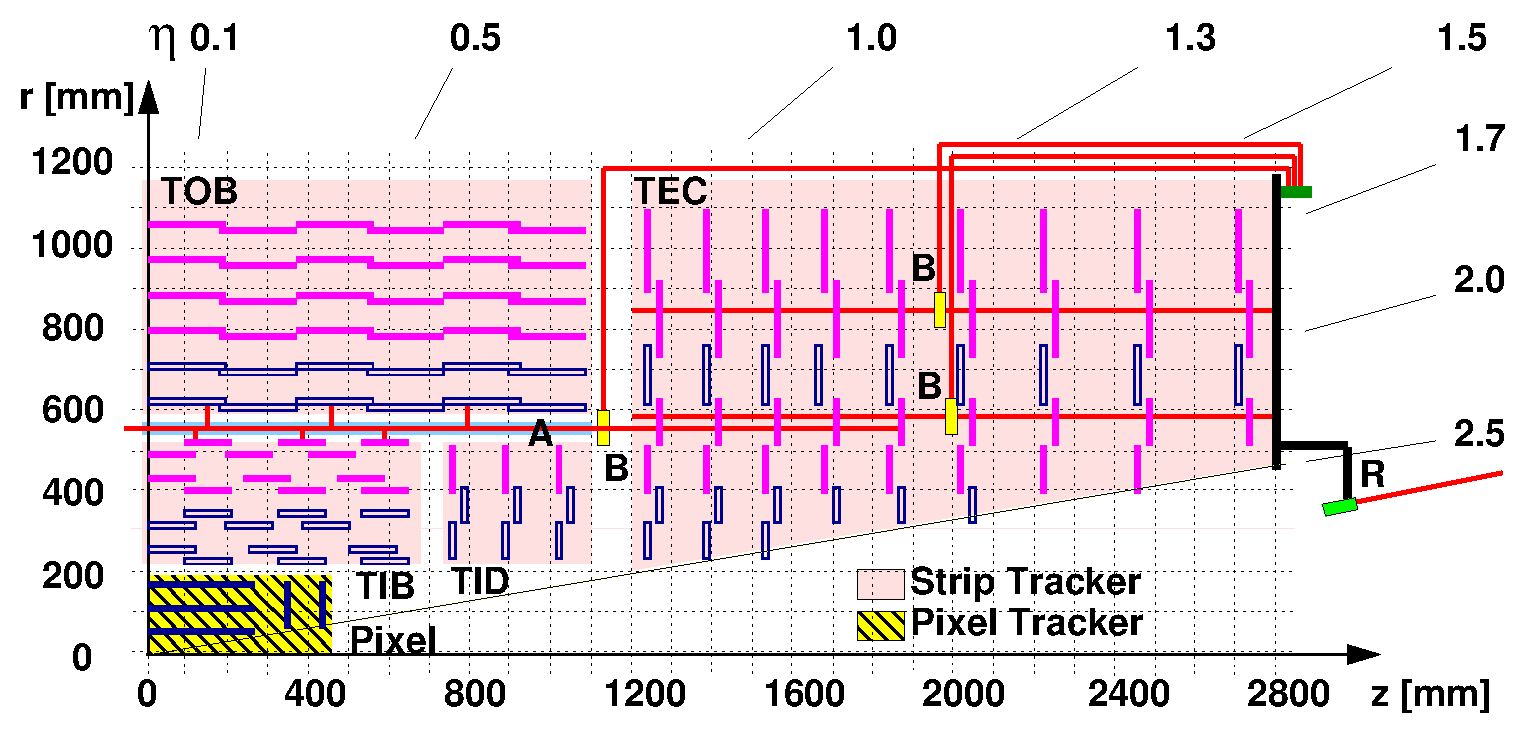
\includegraphics[width=.8\linewidth]{Experiment/figures/TrackerSystemLAS.eps}
\caption[Geometry of the Tracker System]{Tracker cross-section (1/4 of the $z$ view). The pixel tracker is located at the innermost radii of the detector and is labeled in striped yellow. The strip tracker is composed of four regions: Tracker Inner Barrel (TIB), Tracker Outer Barrel (TOB), Tracker End Cap (TEC), and Tracker Inner Disks (TID). The blue pieces are double-sided modules while magenta are single-sided. In addition to the silicon sensors, an infrared laser alignment system is used to provide coarse calibration for the tracker.}
\label{fig:TrackerSystem}
\end{center}
\end{figure}

As particle flux will clearly be highest closest to the interaction point, the smallest elements must be placed to avoid oversaturating the electronics. Silicon pixels of size $100\times150$ $\mu\rm{m}^2$ are arranged in three cylindrical barrel layers at $r=$ 4.4 cm, 7.3 cm, and 10 cm each with a length of 53 cm plus two endcap annuli at $|z|=$ 34.5 and 46.5 cm with radius from $r=$ 6 cm to 15 cm. The pixels are arranged in modules with read-out chips (16 per module in the barrel, 2-10 per module in the endcap), each of which reads the output of an array of $52\times80$ pixels. The output and location of any active pixels are stored in a buffer, awaiting decision to be stored permanently or not from the Level-1 Trigger (see Sec.~\ref{sec:Triggers}).

Outside of the pixel layers, the particle flux will be lower. Tracker elements can be a bit larger without oversaturating, so silicon microstrips are used (minimum cell size of 10 cm $\times$ 80 $\mu$m for $20 < r < 55$ cm and 25 cm $\times$ 180 $\mu$m for $r>55$ cm). The strip tracker is divided into four regions, named to indicate their location in the tracker subsystem: Tracker Inner Barrel (TIB), Tracker Outer Barrel (TOB), Tracker End Cap (TEC), and Tracker Inner Disks (TID). The TIB consist of four layers covering $|z|<$ 65 cm while the TOB covers $|z|<$ 110 cm and is made of six layers. By the orientation and size of the components, the barrel has single-point $r-\phi$ resolution of 23-34 $\mu$m (35-52 $\mu$m) and $z$ resolution of 230 $\mu$m (530 $\mu$m) in the TIB (TOB). For the endcap region, the TID is made of three rings that fill the gap between the TIB and TOB while the TEC is made of 9 rings stretching from $120 < |z| < 280$ cm. As the radiation is even smaller in the outer regions of the tracker, the strips can be longer and thicker. In the TOB and six outermost layers of the TEC, the sensors are slightly thicker at 500 $\mu$m compared to the 320 $\mu$m thick sensors elsewhere. By associating multiple tracker hits, trajectories of charged particles can be constructed. The ultimate designed global track resolution can be seen for muons and pions (the lightest meson) in Fig.~\ref{fig:TrackEfficiency}.

\begin{figure}[htbp]
\begin{center}
\includegraphics[width=.45\linewidth]{Experiment/figures/MuonTrackEfficiency.pdf}
\includegraphics[width=.45\linewidth]{Experiment/figures/PionTrackEfficiency.pdf}
\caption[Global Track Reconstruction Efficiency at CMS]{Global track reconstruction efficiency of muons (left) and pions (right) for transverse momenta of 1, 10, and 100 $\rm{GeV}/c$. Overall efficiency decreases for smaller $p_T$ and near the edges of the detectable region.}
\label{fig:TrackEfficiency}
\end{center}
\end{figure}

As the tracker subsystem is the only one that can reconstruct vertices, great care is taken to affirm that the numerous pieces of the tracker are aligned to very high precision (ideally smaller than the single-point resolution, so $\lesssim10\mu\rm{m}$). After construction, a laser alignment system is used to calibrate the tracker, as well as other subsystems, to account for shifts in orientation. However, this method primarily accounts for large scale structure and not individual module misalignments. In sum, there are 9.6 million strips and 66 million silicon pixels spread across over 16000 modules, where the position and orientation of each must be tracked independently both before and during operation of CMS. The only way to account for all modules and get the desired detector position resolution is to use track-based alignment.

After measuring the positions of the various devices during construction and utilizing the laser alignment system, trajectories of known particles can be used to further the alignment. Since trajectories must be continuous, small misalignments of the modules will appear as discontinuities in the tracks. Looking for these discontinuities and measuring the pull of individual elements, the true orientation can be found.

In 2008, when the detector was fully constructed but the beam was not yet running, millions of cosmic muons were tracked through the detector. Computationally, to find the individual module corrections, it is equivalent to minimizing a matrix equation for $O(10^5)$ degrees of freedom, which is extraordinarily intensive. Nevertheless, using a combined method of algorithms to find global and local correlations, the positions of the modules were determined to an average precision of 3-4 $\mu$m in the barrel and 3-14 $\mu$m in the endcap in their respective most sensitive coordinate~\cite{Chatrchyan:2009sr}. Since environmental conditions of operation can cause deviations over time, similar alignment strategies are used by CMS during data collection.

\subsection{Particle Identification}
\label{sec:ParticleID}

During operation, when the proton beams collide, all of the subsystems work in tandem to identify different particles by what portions they interact with. For example, both muons and electrons will record hits in the tracker, but the muon will move through the muon system while electrons stop in the ECAL. Fig.~\ref{fig:CMSSliceWithTracks} shows a diagram with the expected interactions from a sample set of particles. In theory, it seems like this should be simple categorization: only electrons and photons interact with the ECAL, hadrons will interact with the HCAL, etc. Although it can be this simple, in practice, it is more nuanced. In one crossing, there are roughly 20-30 collisions and each can have multiple decay products which could deposit energies at similar locations; if a photon strikes the ECAL near an electron, how does CMS disentangle the two? Moreover, the lines between what particles interact with which subsystems aren't quite as rigid. Neutral pions will commonly decay to two photons and thus could mimic a photon in the ECAL, for example. Alternatively, an electromagnetic decay in the ECAL can leak into the HCAL. CMS accounts for these \textit{fake rates} and makes proper identifications by using the \textit{particle-flow algorithm}~\cite{ParticleFlowAlgo}. 

\begin{figure}[htbp]
\begin{center}
\includegraphics[width=.9\linewidth]{Experiment/figures/CMSSliceWithTracks.png}
\caption[Trajectories and Decays for Particle Identification in CMS]{Transverse slice of CMS with sample trajectories and decays from expected SM particles. Photons (dashed blue) and electrons will deposit their energy in the Electromagnetic Calorimeter, while both neutral (dashed green) and charged hadrons (green) deposit in the Hadronic Calorimeter. Muons (blue) will move through the muon system. All charged particles will interact with the tracker, leaving curved trajectories.}
\label{fig:CMSSliceWithTracks}
\end{center}
\end{figure}

Particle-flow links the output from the different subsystems to iteratively identify particles. For any charged particles, there will be tracks that should align with energy deposits in the calorimeters or muon system. Any hits in the calorimeters are clustered by looking for local maxima and associating nearby elements that are above threshold. In some cases, additional information can be used with the clustering. For example, in the ECAL, electrons will spread energy over a larger area of crystals that converted photons. These clusters (or trajectories in the muon system) are then matched to trajectories in the tracker system. Starting with a very tight cut between the two elements, matched particles and their associated hits in the subdetectors are removed from consideration and the algorithm repeats with a looser constraint.

This algorithm removes elements in a particular order\footnote{This is roughly in order of resolution for the expected particle, where each identification has little influence on successive identifications.}, starting with global muons, then electrons and photons, and finishing with jets. Once all particles are reconstructed, the missing transverse energy can be calculated. Finally, isolation can be used to indicate whether a given reconstructed particle is \textit{prompt}, meaning that it comes from an initial interaction. These reconstructed particles form the basic framework of all analyses at CMS. 

\subsection{Triggers}
\label{sec:Triggers}

As specified in Sec.~\ref{sec:LHC}, the intended number of collisions is on the order of 1 billion per second. However, even using state-of-the-art storage technology only about 100 events per second can be stored for later analysis, so nearly all of the collisions need to be rejected. Instead of arbitrarily taking data every hundredth of a second, a trigger system is designed so that only potentially interesting events can be captured. To determine what is interesting, data is temporarily stored and filtered by custom electronics. For the first trigger, Level-1, events are only accepted if they either have i) primitive objects from subsystems that pass $p_T$ or $E_T$ thresholds or ii) global $E_T$ or missing transverse energy ($E_T^{miss}$ or MET). The detector elements with fast time resolution, like the RPCs in the muon system (see Sec.~\ref{sec:MuonSystem}), define these primitive objects. Altogether, the Level-1 trigger procedure, including data transfer and decision making, is designed to be completed within 3.2 $\mu\rm{s}$ and reduces the rate of events to approximately 100 kHz.

After passing the Level-1 trigger, high level triggers (HLTs) apply additional processing to further reduce the throughput. Where the Level-1 triggers use primitive objects, HLT cuts on approximately reconstructed objects, applying thresholds for observables like $p_T$, relative isolation in the calorimeters and/or tracker, or $|\eta|$ of the particle. Although a primary purpose of the HLT cuts is to bring the event rate to 100 Hz, these cuts are tuned to be broadly applicable to different analyses, being maximally inclusive to the intended signal while minimizing backgrounds. Each analysis group can then select the data that pass the appropriate high level triggers to make a high precision measurement, exclude a theoretical model, or discover a new as-yet undetected particle.

\section{Summary}
\label{sec:expt_summary}

In 2008, after 25 years of construction, the LHC began operation. Within another two years, the combined energy of the beams reached 7 $\rm{TeV}$. In 2011, over 5 $\mathrm{fb}^{-1}$ was collected for 7 $\rm{TeV}$. After increasing the energy to 8 $\rm{TeV}$ in 2012, nearly another 20 $\mathrm{fb}^{-1}$ was collected. This was sufficient to confirm the existence of a Higgs-like boson, appearing to achieve one of the most elusive discoveries in particle physics. This chapter has reviewed the intricacies of the CMS detector itself, explaining the mechanism used to extract relevant information from the decays of trillions of high energy proton collisions. But how exactly was the new particle found in this mountain of data? How well can we measure its properties? Put bluntly, is this really the Higgs we've been looking for?